\section{Project Structure}

We use, as already mentioned, two GIT repositories, LpzRobots and GoRobots.

Later, the controllers for each robot will be implemented within \emph{GoRobots}, accessing the robots, which are located in \emph{LpzRobots}. The folder \emph{DEMO} will later contain demos of the different robots.
Another visualisation of the two repositories and where which file belongs is given in Figure \ref{struc2}.
\begin{figure}[h!]
 \begin{center}
  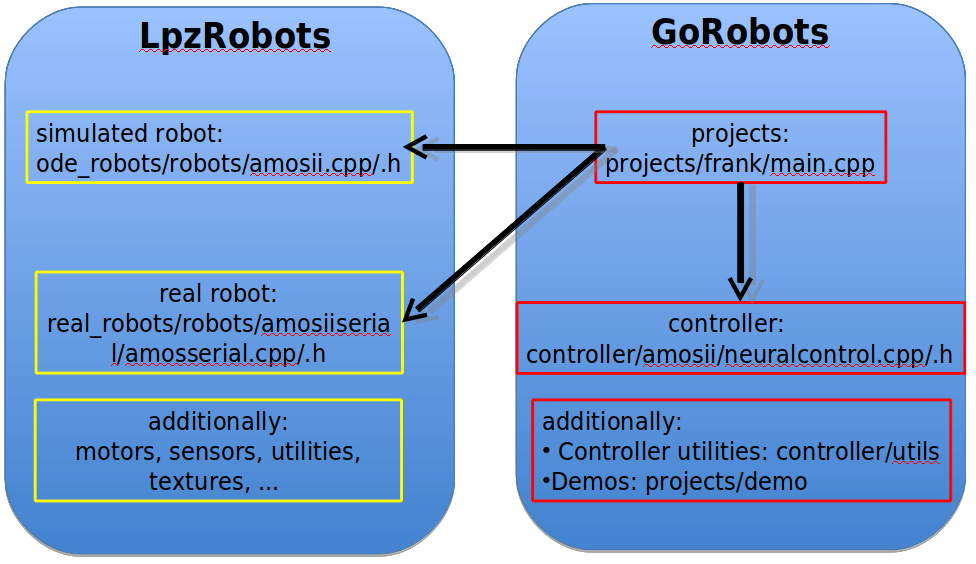
\includegraphics[width=10cm]{./pics/struct.png}
 \end{center}
\caption{Structure of the two repositories, LpzRobots and GoRobots}
\label{struc2}
\end{figure}

You will later work with your own copy of the two repositories.

\newpage

\begin{figure}[h!]
 \begin{center}
  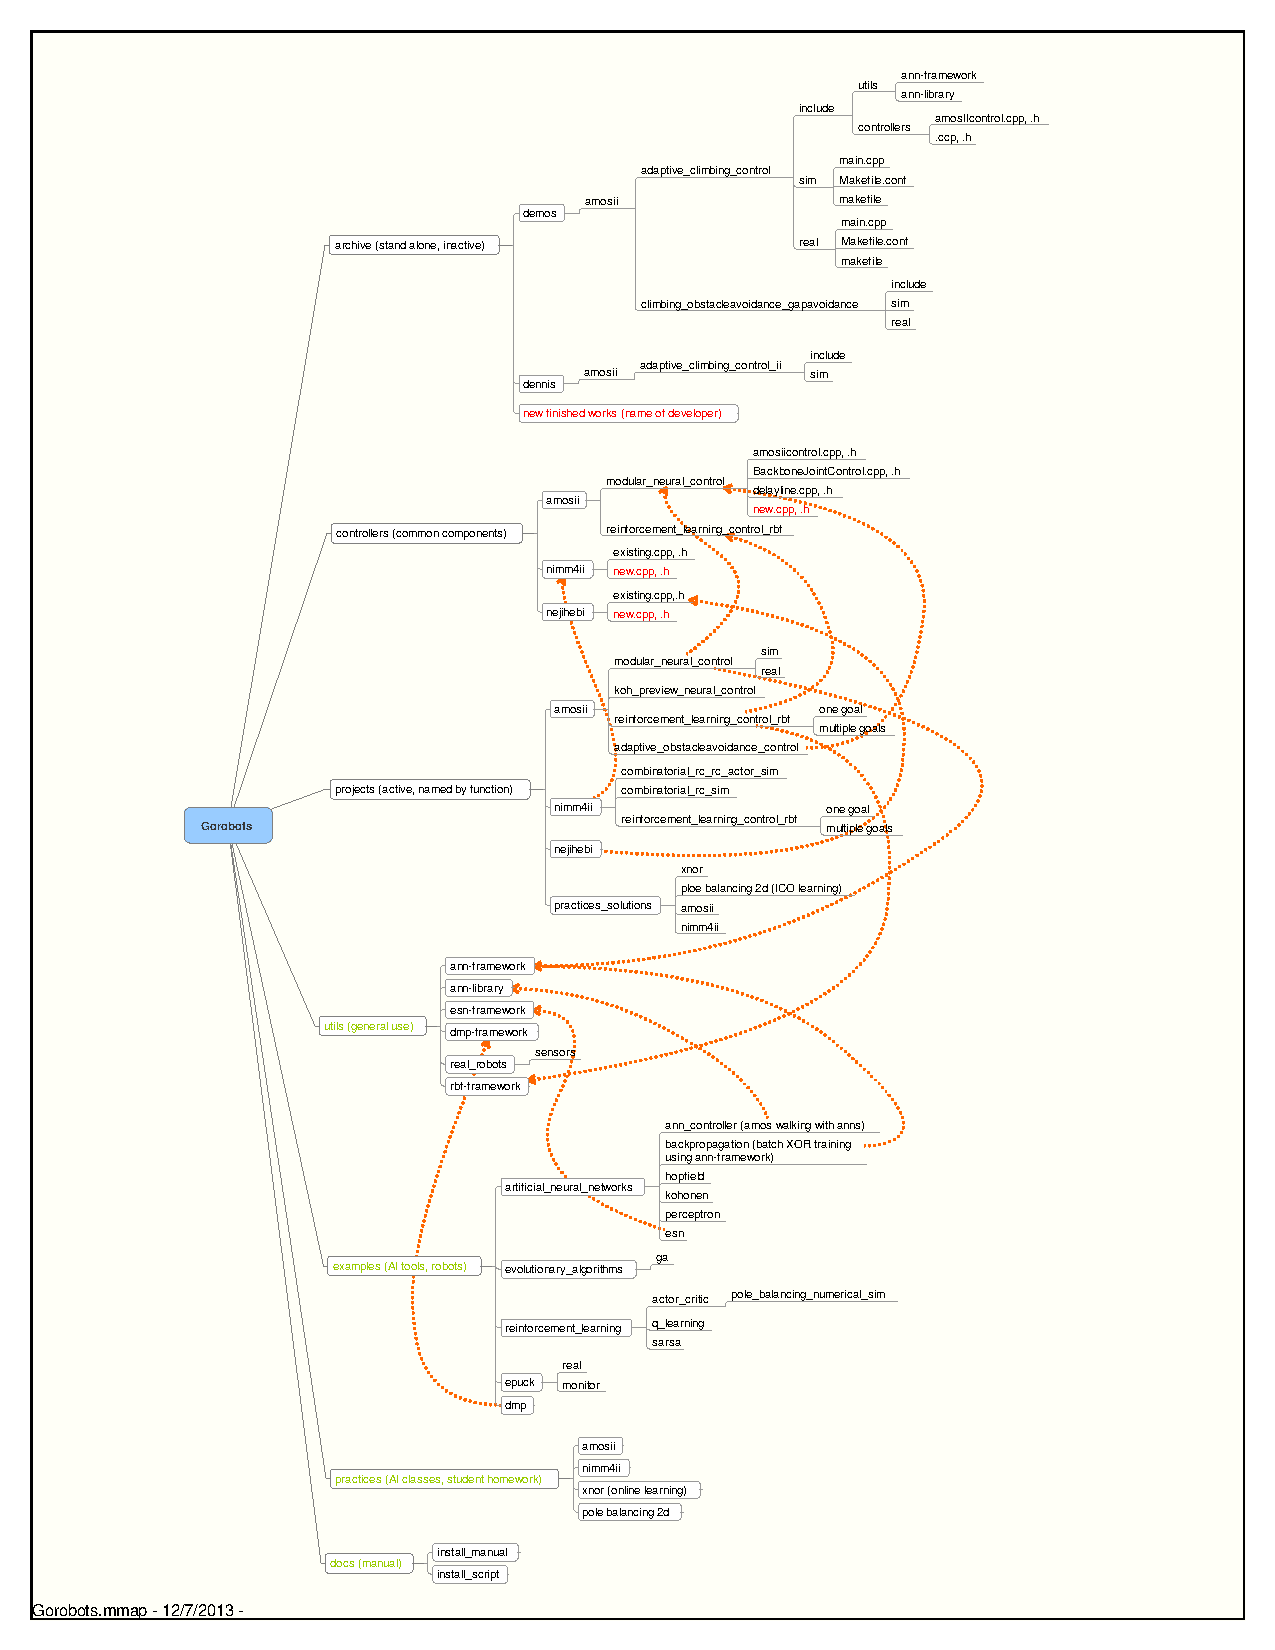
\includegraphics[width=14cm]{./pics/Gorobots.pdf}
 \end{center}
\caption{Structure of GoRobots. Green parts belong to GoRobotsEdu}
\label{struc3}
\end{figure}
